\documentclass{article}
\usepackage{amsmath}
\usepackage{amssymb}
\usepackage{graphicx}
\usepackage{hyperref}
\usepackage[version=4]{mhchem}

\title{Problem 1}
\date{}

\begin{document}
\maketitle

\section*{Problem}
Circle \(O\) of radius 45 is inscribed in equilateral triangle \(A B C\). Circle \(P\) is tangent to circle \(O\) and segments \(A B\) and \(B C\). Find the area of circle \(P\).\\
(A) \(245 \pi\)\\
(B) \(625 \pi\)\\
(C) 225\\
(D) \(225 \pi\)\\
(E) 700\\
\centering
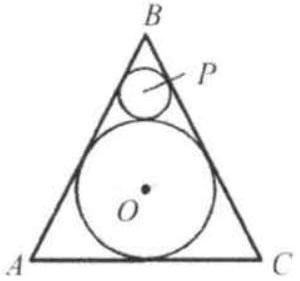
\includegraphics[width=\textwidth]{images/problem_image_1.jpg}

\section*{Solution}
(D).\\
Draw \(P F \perp A B\) and \(O E \perp A B\).\\
Connect \(B D\).

Triangle \(B E O\) is a \(30^{\circ}-60^{\circ}-90^{\circ}\) triangle and \(B O=2 O E\). \(O E=45\) and \(B O=2 O E=90\), and \(B D=90+45=135\).\\
Let \(P F=r\).\\
\centering
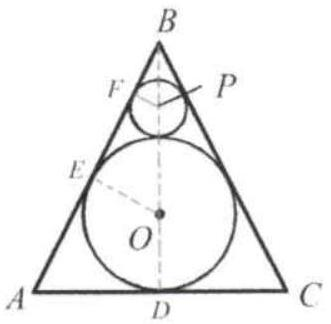
\includegraphics[width=\textwidth]{images/reasoning_image_1.jpg}

Triangle \(B F P\) is a \(30^{\circ}-60^{\circ}-90^{\circ}\) triangle and \(B P=2 r\).\\
In other word, \(B P=B O-45-r\).

So \(2 r=B O-45-r \quad \Rightarrow 3 r=90-45=45\).\\
So \(r=15\).

The area is \(\pi(15)^{2}=225 \pi\).

\end{document}
